\documentclass[10pt, conference, a4paper, onecolumn, compsocconf]{IEEEtran}

\usepackage[utf8]{inputenc}
\usepackage[]{algorithm2e}
\usepackage{gensymb}
\usepackage{amssymb}
\usepackage{amsmath}
\usepackage{graphicx}
\usepackage{caption}
\usepackage{subcaption}
\usepackage{wrapfig}
\usepackage{url}
\usepackage{hyperref}
\usepackage{float}
\usepackage{xcolor}
\usepackage{listings}
% \usepackage{authblk}

\begin{document}

\title{A Collaborative Filtering Based Movie Recommendation System}

\author{
\authorblockN{PETROVA Kalina}
\authorblockA{Department of Computer Science, \\ETH Zurich, Switzerland\\Email: kpetrova@student.ethz.ch}
\and
\authorblockN{IVANOV Petar}
\authorblockA{Department of Computer Science, \\ETH Zurich, Switzerland\\Email: ivanovpe@student.ethz.ch}
\and
\authorblockN{LI Shiyi}
\authorblockA{Department of Earth Sciences, \\ETH Zurich, Switzerland\\Email: lishi@student.ethz.ch}
}

\specialpapernotice{\textit{Computational Intelligence Lab, Spring 2018}\\\today}
% \pudid{}
\maketitle

\begin{abstract}
This is the abstract
\end{abstract}

\section{Introduction}
\label{sec:introduction}

Here is the introduction.

\section{Methods}
\label{sec:methods}

Hello I am figures and algorithms

\begin{figure}
\begin{flalign*}
K_{\text{diamond}} &= \begin{bmatrix}0 & 0.25 & 0 \\ 0.25 & 0 & 0.25 \\ 0 & 0.25 & 0\end{bmatrix}\\
%K_{\text{gauss}} &= \begin{bmatrix}0.011 & 0.084 & 0.011\\0.084 & 0.620 & 0.084 \\0.011 & 0.084 & 0.011\end{bmatrix}\\
K_{\text{diag}} &= \begin{bmatrix}0.38 & 0.04 & 0.04 \\ 0.04 & 0 & 0.04 \\ 0.04 & 0.04 & 0.38\end{bmatrix}
\end{flalign*}
\caption{Kernels used for diffusion.}
\label{fig:kernels}
\end{figure}

\begin{algorithm}
	\KwIn{Image $I$, mask $M$, kernel $K$ and threshold $\epsilon$}
	\KwResult{Reconstructed image $I_{r}$}
	$K \leftarrow \frac{K}{\sum_i \sum_j K_{i,j}}$ (normalize $K$ to preserve energy)\; 
	$I_{prev} \leftarrow 0_{size(I)}$\;
	$I_{r} \leftarrow I$\;
	\While{$\|I_{r} - I_{prev} \|_{F} > \epsilon$}{
		$I_{prev} \leftarrow I_{r}$\;
		$I_{r} \leftarrow \text{convolve}(I_{r}, K)$\;
		$I_{r} \leftarrow I_{r} \circ \mathbf{1}_{M = 0} + I \circ \mathbf{1}_{M \neq 0}$ \;
	}
	\quad
\caption{Diffusion algorithm for inpainting. We denote element-wise multiplication with the $\circ$ operator. The $\mathbf{1}_{M=0}$ function represents a matrix with elements $(i,j)$ set to 1 when $M_{i,j}=0$ and 0 otherwise.}
\label{alg:diffusion}
\end{algorithm}

\begin{figure}
	\centering
	\begin{subfigure}[b]{0.4\textwidth}
		\centering
		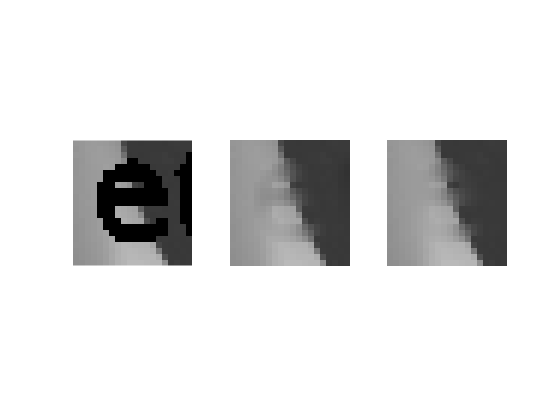
\includegraphics[clip, trim=0cm 5.2cm 0cm 4cm, width=0.85\textwidth]{figures/step-by-step-cross}
		\caption{Diamond kernel $K_{\text{diamond}}$}
		\label{fig:stepbystepcross}
	\end{subfigure}
	\begin{subfigure}[b]{0.4\textwidth}
		\centering
		
\includegraphics[clip, trim=0cm 5.2cm 0cm 4cm, width=0.85\textwidth]{figures/step-by-step-directional}
		\caption{Directional kernel $K_\theta$ for $\theta = 100\degree$.}
		\label{fig:stepbystepdir}
	\end{subfigure}
	\caption{Step-by-step illustration of the diffusion process with different kernels. Each step represent 20 iterations.}
\end{figure}





\subsubsection{Constructing a directional kernel}

I am a subsubsection

\subsubsection{Per-patch diffusion using $K_\theta$}

I am another subsubsection.



\section{Results}
\label{sec:results}

This is results. 

Example of list:

\begin{enumerate}
	\item Sparse-coding with a DCT dictionary \cite{cildct}.
	\item Sparse-coding with a Haar wavelet \cite{cilhaar}.
	\item Singular Value Decomposition \cite{cilsvd}.
	\item Regular diffusion with a $K_{\text{diamond}}$ kernel.
	\item Directional diffusion with patches of size $16 \times 16$.
	\item Directional diffusion with patches of size $32 \times 32$.
\end{enumerate}

blabblabla: 
\begin{flalign*}
\text{MSE}(I, I^{\text{rec}}) = \frac{1}{512 \cdot 512} \sum_{i,j} (I_{i,j} - I^{\text{rec}}_{i,j})^2
\end{flalign*}


Hello I am a table
\begin{table}
	\centering
	\begin{tabular}{|l|c|c|}
		\hline
		\textbf{Algorithm} & \textbf{MSE} & \textbf{Runtime} \\ \hline \hline
		Directional Diffusion ($16 \times 16$) & $\mathbf{0.00055} \pm 0.00051$ & $8.7 \pm 2.13$ \\ \hline
		Directional Diffusion ($32 \times 32$) & $0.00057 \pm 0.00053$ & $2.4 \pm 0.04$ \\ \hline
		Diffusion ($K_{\text{diamond}}$) & $0.00061 \pm 0.00057$ & $\mathbf{0.5} \pm 0.06$ \\ \hline
		Sparse-coding (DCT) & $0.0015 \pm 0.0012$ & $12.8 \pm 4.67$ \\ \hline
		Sparse-coding (Haar wavelet) & $0.0024 \pm 0.0021$ & $13.0 \pm 3.72$ \\ \hline
		Singular Value Decomposition & $0.0019 \pm 0.0018$ & $0.7 \pm 0.09$ \\ \hline
	\end{tabular}
	\caption{Mean squared error and runtime (in seconds) across different algorithms for the text mask. The best result is highlighted in bold.}
	\label{tbl:err_text}
\end{table}


\section{Discussion}
\label{sec:discussion}

why?

because sky is high!

\section{Conclusion}
\label{sec:conclusion}

U are close




\bibliographystyle{IEEEtran}
\bibliography{cil_report}

\end{document}
